% partes/parte1/cap02.tex
\chapter{Perfil, segmentación y mercado meta digital}
\label{cap:02}

\begin{cajaFicha}
\begin{description}
  \item[Unidad temática] I — Comportamiento, perfil y gestión de datos del consumidor digital.
  \item[Temas del programa] 1.2 Perfil del consumidor digital: 1.2.1 Segmentación del mercado digital y variables; 1.2.2 Mercado meta o target digital; 1.2.3 Tipos de perfil del consumidor digital; 1.2.4 Radiografía del consumidor digital en México y el mundo; 1.2.5 Diversidad de perfiles de consumidor digital por modelo de negocios-industria.
  \item[Horas] Teoría 2.0 · Práctica 3.0 · Aprendizaje autónomo 2.0.
  \item[Competencia de la unidad] Identifica el comportamiento del consumidor digital y su evolución a partir de sus tipos de perfil y gestión de datos.
  \item[Resultados de aprendizaje observables] Al concluir el capítulo, el estudiante:
  \begin{enumerate}
    \item aplica el proceso de segmentación-targeting-posicionamiento a un caso de mercado digital;
    \item distingue segmentación rígida de segmentación difusa y justifica cuándo cada una es preferible;
    \item describe, con datos verificados, la radiografía del consumidor digital mexicano frente al panorama internacional.
  \end{enumerate}
  \item[Prerrequisitos] Cap. 1 (evolución del consumidor digital).
\end{description}
\end{cajaFicha}

\section{Caso de apertura}

Una misma persona puede ser, para una plataforma de streaming, un
\enquote{usuario ocasional de fin de semana}, y para una app bancaria, un
\enquote{usuario de alto compromiso}. No hay contradicción: son dos negocios
midiendo comportamientos distintos sobre la misma persona. El error común de
la segmentación de manual es tratar al consumidor como si tuviera una sola
identidad de compra fija, aplicable a cualquier categoría. Este capítulo
propone lo contrario: el perfil de un consumidor digital es específico del
comportamiento que se mide, y —como se verá en el laboratorio— muchas veces
ni siquiera es una etiqueta única dentro de esa misma categoría.

\section{Desarrollo teórico}

\subsection{Segmentación del mercado digital y sus variables}
\progtag{1.2.1}

La segmentación de mercado tiene una fuente académica precisa: Wendell R.
Smith, quien en 1956 la definió, en contraste con la diferenciación de
producto, como la estrategia de \enquote{ver un mercado heterogéneo (...) como
un número de mercados homogéneos más pequeños, en respuesta a preferencias de
producto diferentes entre segmentos importantes del mercado}
\parencite{smith1956}. Sobre esa base se construyó, décadas después, el
proceso que hoy se enseña como estándar: Segmentación, Targeting y
Posicionamiento (STP), sistematizado en los manuales de Philip Kotler
\parencite{kotler2021marketing50}
(figura~\ref{fig:cap02-stp}).

\begin{figure}[htbp]
  \centering
  % figuras/tikz/cap02-stp.tex
% Proceso STP (Segmentación - Targeting - Posicionamiento), sistematización
% posterior construida sobre la base conceptual de Smith (1956).
\begin{tikzpicture}[
    etapa/.style={rectangle, rounded corners, draw=guindaIPN, thick, fill=guindaIPNClara,
                  minimum width=3.4cm, minimum height=1.6cm, align=center, font=\small},
    flecha/.style={-{Stealth[length=3mm]}, thick, draw=doradoIPN},
    nota/.style={font=\scriptsize, text width=3.4cm, align=center}
  ]
  \node[etapa] (s) at (0,0) {\textbf{Segmentación}\\ agrupar por\\ variables comunes};
  \node[etapa] (t) at (4.6,0) {\textbf{Targeting}\\ elegir el o los\\ segmentos meta};
  \node[etapa] (p) at (9.2,0) {\textbf{Posicionamiento}\\ definir el lugar\\ en la mente del\\ segmento meta};

  \draw[flecha] (s) -- (t);
  \draw[flecha] (t) -- (p);

  \node[nota] at (0,-1.4) {Smith (1956): base conceptual};
  \node[nota] at (4.6,-1.4) {Mercado meta o \textit{target}};
  \node[nota] at (9.2,-1.6) {Sistematización posterior (manuales de Kotler)};
\end{tikzpicture}

  \caption{El proceso STP como sistematización posterior de la base
  conceptual de Smith (1956). Fuente: elaboración propia.}
  \label{fig:cap02-stp}
\end{figure}

Las variables clásicas de segmentación —geográfica, demográfica,
psicográfica y conductual—, sistematizadas en la bibliografía de
comportamiento del consumidor \parencite{hoyer2024consumer}, no
desaparecieron con la digitalización; se
volvieron medibles con una granularidad que antes era impensable. El
cuadro~\ref{tab:cap02-variables} contrasta la versión analógica de cada
variable con su equivalente digital.

\begin{table}[htbp]
\centering
\begin{tabular}{@{}p{2.6cm}p{4.6cm}p{5.4cm}@{}}
\toprule
Variable & Versión clásica (encuesta/censo) & Equivalente digital (dato conductual) \\
\midrule
Geográfica & Región, ciudad declarada & Geolocalización de dispositivo, dirección IP, zona de entrega \\
Demográfica & Edad, sexo, ingreso declarados & Edad/sexo inferidos por plataforma, nivel socioeconómico por comportamiento de compra \\
Psicográfica & Estilo de vida, valores (encuesta) & Intereses inferidos por interacción con contenido, seguimiento de cuentas \\
Conductual & Frecuencia de compra declarada & Frecuencia, recencia y monto de transacción, registrados directamente \\
\bottomrule
\end{tabular}
\caption{Variables de segmentación: versión clásica vs. equivalente digital.
Fuente: elaboración propia con base en la tradición de Smith (1956) y su
sistematización en la bibliografía de comportamiento del consumidor
\parencite{smith1956,solomon2017}.}
\label{tab:cap02-variables}
\end{table}

La columna derecha explica, mejor que cualquier definición abstracta, por
qué la segmentación digital es distinta en grado, no en naturaleza: la
variable conductual —antes la más difícil y cara de medir, porque dependía
de que el consumidor recordara y declarara su propio comportamiento— es hoy
la más barata de obtener, porque el sistema la registra directamente. Este
cambio de costo relativo entre tipos de variable es, en buena medida, la
verdadera revolución detrás de \enquote{segmentar en la era digital}: no es que
existan variables nuevas, es que la variable antes más cara ahora es casi
gratuita.

\subsection{Mercado meta o \textit{target} digital}
\progtag{1.2.2}

Definir el mercado meta es elegir, de entre los segmentos identificados,
aquel o aquellos hacia los que la organización dirige su oferta y su
comunicación. En el entorno digital esta decisión tiene una consecuencia
operativa directa que no existía en medios masivos: el mercado meta no solo
se declara en un plan de mercadotecnia, también se \textit{configura} en
cada plataforma publicitaria —audiencias personalizadas, públicos similares
(\textit{lookalike}), exclusiones— como parámetros técnicos que determinan a
quién exactamente se le muestra un anuncio. Elegir mal el mercado meta ya no
es solo un error estratégico: es, literalmente, un parámetro mal configurado
que desperdicia presupuesto en cuestión de horas.

\subsection{Tipos de perfil del consumidor digital}
\progtag{1.2.3}

Al preparar este capítulo se buscó, de forma deliberada, una tipología
académica de \enquote{tipos de perfil del consumidor digital} atribuible con
precisión a un autor de la bibliografía oficial —se revisaron, entre otras,
las ediciones más recientes de Solomon \parencite{solomon2023consumer} y de
Hoyer, MacInnis y Pieters \parencite{hoyer2024consumer}—. No se encontró una:
las clasificaciones populares que circulan en blogs de mercadotecnia en
español
(\enquote{el informado}, \enquote{el social}, \enquote{el impulsivo}) no tienen
aparato metodológico documentado ni autoría rastreable. La fuente de la
bibliografía oficial que sí desarrolla una tipología estructurada es
\textit{El Cubo NORISO}, de Delgado Soriano, Bonet, Deza y Fernández
García-Andrade \parencite{delgado2015noriso}, que propone ocho perfiles de
personalidad del consumidor digital construidos sobre un modelo propio. Este
capítulo recomienda esa fuente para el desarrollo del tema en la exposición
del equipo (§7), con una advertencia: es una tipología de autor, de
divulgación, no revisada por pares —debe presentarse como tal, distinta de
un hallazgo científico, exactamente con el mismo criterio que el capítulo~1
aplicó a la serie \textit{Marketing X.0}.

Lo que sí tiene respaldo metodológico sólido no es una tipología cerrada de
perfiles, sino el método para construirla: el clustering. La
sección~\ref{sec:cap02-lab} desarrolla dos variantes —rígida y difusa— con
las que cualquier organización puede construir su propia tipología de
perfiles a partir de datos propios, en vez de adoptar una tipología genérica
de manual.

\begin{figure}[htbp]
  \centering
  % figuras/tikz/cap02-rigida-vs-difusa.tex
% Contraste conceptual: segmentación rígida (pertenencia binaria, k-means)
% vs. segmentación difusa (pertenencia parcial, fuzzy c-means).
\begin{tikzpicture}[
    seg/.style={circle, draw=guindaIPN, thick, fill=guindaIPNClara, minimum size=2.6cm, font=\scriptsize, align=center},
    segb/.style={circle, draw=bronceIPN, thick, fill=bronceIPNClaro, minimum size=2.6cm, font=\scriptsize, align=center},
    punto/.style={circle, fill=black, minimum size=3pt, inner sep=0pt},
    titulo/.style={font=\small\bfseries}
  ]
  % Panel izquierdo: segmentación rígida
  \node[titulo] at (0,2.2) {Rígida ($k$-means)};
  \node[seg] (A1) at (-1.1,0) {Segmento A};
  \node[segb] (B1) at (1.5,0) {Segmento B};
  \node[punto] (p1) at (0.15,0.15) {};
  \node[font=\tiny, align=center] at (0.15,-0.55) {consumidor $i$\\ pertenece solo a A};

  % Panel derecho: segmentación difusa
  \begin{scope}[xshift=6.5cm]
    \node[titulo] at (0,2.2) {Difusa (\textit{fuzzy c-means})};
    \node[seg, opacity=0.75] (A2) at (-0.9,0) {Segmento A};
    \node[segb, opacity=0.75] (B2) at (0.9,0) {Segmento B};
    \node[punto] (p2) at (0,0.1) {};
    \node[font=\tiny, align=center] at (0,-0.85) {consumidor $i$: $u_{iA}=0.63$,\\ $u_{iB}=0.37$};
  \end{scope}
\end{tikzpicture}

  \caption{Segmentación rígida (pertenencia binaria) vs. difusa (pertenencia
  parcial, con grados $u_{iA}$ y $u_{iB}$ que suman 1). Fuente: elaboración
  propia.}
  \label{fig:cap02-rigida-difusa}
\end{figure}

\begin{cajaFrontera}
\textbf{Segmentación difusa: pertenencia parcial en vez de casillas
rígidas.} La segmentación tradicional asigna a cada consumidor un único
segmento, como si las fronteras entre grupos fueran nítidas. El algoritmo
\textit{fuzzy c-means} (FCM), formalizado por Bezdek
\parencite{bezdek1981} sobre la base de los conjuntos difusos de Zadeh
(1965), sustituye esa asignación binaria por un grado de pertenencia
$u_{ik} \in [0,1]$ de cada consumidor $i$ a cada segmento $k$, con la
restricción $\sum_k u_{ik} = 1$. La segmentación rígida (\textit{k-means})
es, en este marco, el caso límite en que toda la pertenencia se concentra en
un solo segmento —no al revés: la difusa es la formulación general; la
rígida, el caso particular simplificado. El laboratorio de este capítulo
implementa ambas sobre el mismo conjunto de datos para que la diferencia sea
observable, no solo declarada.
\end{cajaFrontera}

\subsection{Radiografía del consumidor digital en México y el mundo}
\progtag{1.2.4}
\label{sec:cap02-radiografia}

\begin{table}[htbp]
\centering
\begin{tabular}{@{}lrr@{}}
\toprule
Grupo de edad & Uso diario de internet (h) & Adopción de internet \\
\midrule
18--24 años & 5.7 & — \\
25--34 años & 5.6 & — \\
35--44 años & 4.7 & — \\
55--64 años & 3.2 & — \\
65 años y más & 3.0 & 42.1\,\% \\
\midrule
Zona urbana & — & 86.9\,\% \\
Zona rural & — & 68.5\,\% \\
\bottomrule
\end{tabular}
\caption{Radiografía del consumidor digital mexicano por edad y por zona,
2024. Fuente: elaboración propia con datos de INEGI, ENDUTIH 2024, Reporte de
Resultados 9/25 y Comunicado 57/25 \parencite{inegi2025endutih}.}
\label{tab:cap02-radiografia}
\end{table}

El cuadro~\ref{tab:cap02-radiografia} muestra algo que ninguna tipología de
perfil genérica captura bien: la variable con mayor poder explicativo del
comportamiento digital mexicano no es una categoría psicográfica sofisticada,
es la edad, y de forma casi monótona —a menor edad, más horas de conexión
diaria, con una caída sostenida a partir de los 35 años—. La brecha
urbano-rural (18.4 puntos porcentuales) es la segunda variable con mayor
poder explicativo verificado en este capítulo. Cualquier ejercicio de
segmentación digital en México que ignore estas dos variables estructurales
para saltar directo a variables psicográficas más vistosas corre el riesgo
de sobreajustar categorías elegantes sobre una base demográfica que ya
explica buena parte de la varianza.

\subsection{Diversidad de perfiles por modelo de negocio e industria}
\progtag{1.2.5}

Un mismo consumidor genera perfiles distintos según el modelo de negocio que
lo observa —idea consistente con el enfoque de Sheth y Jain
\parencite{sheth2026} de organizar el comportamiento digital por mecanismos
de datos en vez de por categorías fijas de persona—, porque cada modelo mide
una variable de éxito distinta: una
plataforma de comercio electrónico optimiza por conversión y ticket
promedio; una red social, por tiempo de permanencia y tasa de interacción;
una fintech, por frecuencia de uso y profundidad de producto (cuántos
productos financieros distintos usa la misma persona). No existe, por lo
tanto, un \enquote{perfil digital} único y portable de un consumidor entre
industrias: el perfil es una función del negocio que lo construye, no un
atributo fijo de la persona. Esta idea retoma la distinción persona/dato del
capítulo~1 (figura~\ref{fig:cap01-doble-naturaleza}) y la hace operativa:
cuantos más negocios observan al mismo consumidor, más perfiles distintos y
parciales de esa persona existen, ninguno de ellos completo.

\section{Laboratorio MATLAB: segmentación rígida y difusa}
\label{sec:cap02-lab}

\begin{cajaLaboratorio}
\textbf{Objetivo.} Comparar segmentación rígida (\textit{k-means}) contra
segmentación difusa (\textit{fuzzy c-means}) sobre un conjunto de datos
sintéticos de comportamiento de consumidor digital, e identificar qué
proporción de consumidores queda mal representada por una asignación única
de segmento.

\textbf{Concepto detrás del código.} \textit{k-means} minimiza la suma de
distancias al cuadrado entre cada punto y el centro de su segmento asignado,
con pertenencia binaria. \textit{Fuzzy c-means} minimiza una función
objetivo equivalente pero ponderada por el grado de pertenencia elevado a un
exponente difuso $m$ (aquí $m=2$, valor estándar):
\[
  J_m = \sum_{i=1}^{n}\sum_{k=1}^{c} u_{ik}^{m}\, \lVert x_i - v_k \rVert^2,
  \qquad \text{sujeto a } \sum_{k=1}^{c} u_{ik} = 1 \ \ \forall i,
\]
donde $x_i$ es el vector de comportamiento del consumidor $i$, $v_k$ el
centro del segmento $k$ y $u_{ik}$ su grado de pertenencia. La calidad de la
segmentación rígida se evalúa con el coeficiente de silueta (compara la
distancia de cada punto a su propio segmento contra la distancia al segmento
más cercano); la segmentación difusa se evalúa, en este script, con la
proporción de consumidores cuya pertenencia máxima no supera 0.6 —una forma
directa de cuantificar cuántos casos la segmentación rígida está forzando a
una casilla que no les queda bien.

\textbf{Script.} \texttt{matlab/cap02/cap02\_segmentacion.m}. Es el
\textbf{mismo script, sin modificar}, que se usa en la Práctica 1 de esta
Parte. Genera consumidores \textbf{sintéticos} (\texttt{rng(42)}) con tres
variables de comportamiento (frecuencia de compra mensual, ticket promedio,
engagement digital) a partir de los arquetipos que el estudiante defina en
el bloque de parámetros —tantas filas como arquetipos quiera simular—; el
resto del script (estandarización, k-means, fuzzy c-means, figuras) se
ajusta automáticamente al número de filas que haya.

\begin{lstlisting}[style=MATLABStyle, caption={Bloque de parámetros editable (\texttt{cap02\_segmentacion.m}) — cada fila es un arquetipo.}]
centrosTipicos = [
    1.5,  350,  25    % arquetipo 1: "ocasional"
    4.0,  900,  78    % arquetipo 2: "leal"
    2.6,  600,  52 ]; % arquetipo 3: "intermedio" (traslape deliberado)
dispersionTipica = [ ... ];   % dispersion de cada arquetipo (misma forma)
nClientesPorSegmento = 80;    % tamano de muestra sintetica por arquetipo
\end{lstlisting}

\textbf{Salida esperada.} Al correr el script se imprime la silueta promedio
de k-means y el porcentaje de consumidores con pertenencia difusa ambigua, y
se generan dos figuras: comparación de dispersión k-means vs. fuzzy c-means
(figura~\ref{fig:cap02-comparacion}) y perfil de los segmentos en radar
(figura~\ref{fig:cap02-radar}), ambas con el número de arquetipos usado en
el título.

\begin{center}
  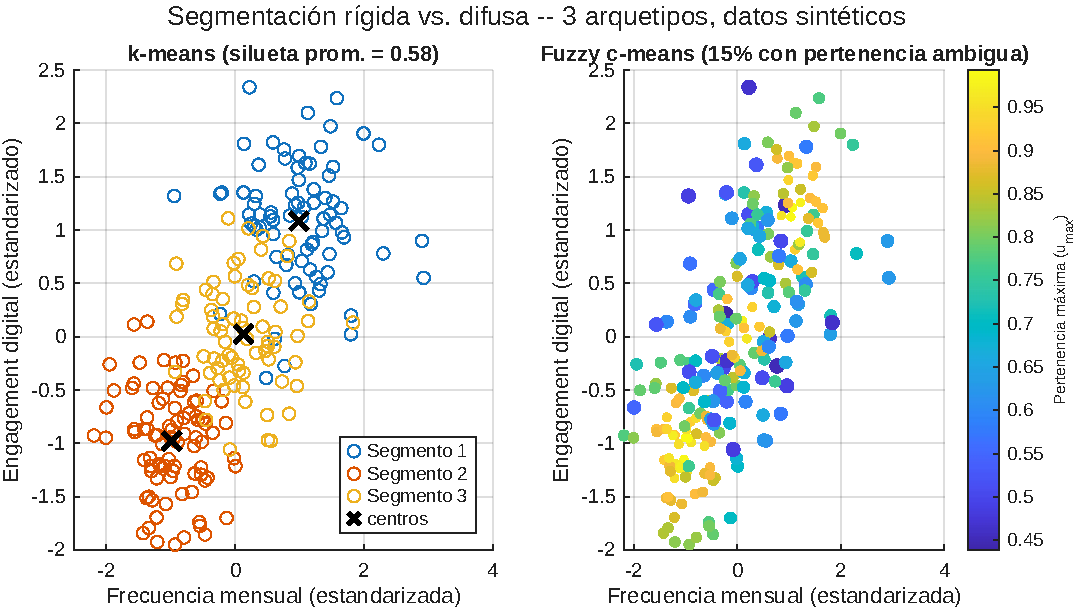
\includegraphics[width=0.98\textwidth]{figuras/matlab/cap02_segmentacion_comparacion.pdf}
  \captionof{figure}{Segmentación rígida (silueta promedio 0.58) vs. difusa
  (15\,\% de consumidores sin pertenencia dominante), con los tres arquetipos
  por defecto del script. Fuente: elaboración propia con datos sintéticos,
  \texttt{rng(42)}.}
  \label{fig:cap02-comparacion}
\end{center}

\begin{center}
  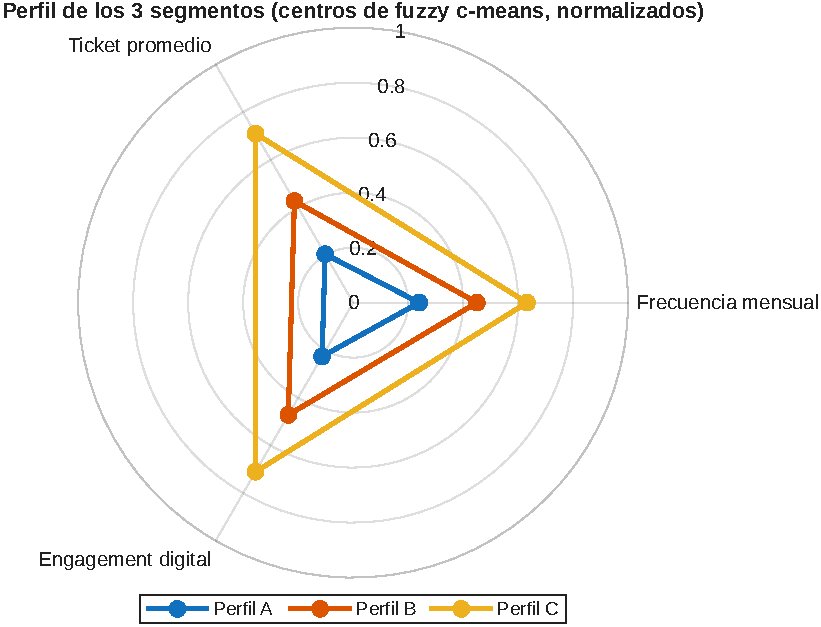
\includegraphics[width=0.62\textwidth]{figuras/matlab/cap02_perfiles_radar.pdf}
  \captionof{figure}{Perfil de los tres segmentos identificados por fuzzy
  c-means, centros normalizados, misma corrida. Fuente: elaboración propia
  con datos sintéticos.}
  \label{fig:cap02-radar}
\end{center}

\textbf{Interpretación de negocio.} El 15\,\% de los consumidores sintéticos
sin pertenencia dominante (figura~\ref{fig:cap02-comparacion}, panel
derecho, puntos de color intermedio y mayor tamaño) son, en términos de
negocio, los casos donde una campaña dirigida \enquote{solo al segmento leal} o
\enquote{solo al segmento ocasional} tiene la mayor probabilidad de desperdicio:
ese consumidor no es completamente ninguno de los dos, y tratarlo como si lo
fuera —en cualquiera de las dos direcciones— es un error de segmentación
sistemático, no aleatorio. El perfil C de la figura~\ref{fig:cap02-radar}
domina las tres variables simultáneamente: es el segmento \enquote{leal} de
alto valor, y su combinación de alta frecuencia, alto ticket y alto
engagement lo hace, en cualquier negocio real, el segmento prioritario de
retención.

\textbf{Ejercicio propuesto (usen exactamente este script, solo cambien el
bloque de parámetros).} Corran el script tres veces y completen un cuadro
con la silueta promedio y el \% de pertenencia ambigua de cada corrida:
\begin{enumerate}
  \item \textbf{Caso A — arquetipos por defecto:} los tres del script
  (\enquote{ocasional}, \enquote{leal}, \enquote{intermedio}).
  \item \textbf{Caso B — más traslape:} acerquen los tres centros entre sí
  (por ejemplo, reduzcan a la mitad la distancia entre las filas de
  \texttt{centrosTipicos}) sin cambiar las dispersiones.
  \item \textbf{Caso C — cuatro arquetipos:} agreguen una cuarta fila a
  \texttt{centrosTipicos} y a \texttt{dispersionTipica} con un arquetipo
  propio, y corran de nuevo.
\end{enumerate}
Con el cuadro completo, respondan por escrito: ¿qué le pasa a la silueta
promedio de k-means cuando los segmentos se acercan (Caso B)? ¿Qué le pasa
al \% de pertenencia ambigua? ¿Mejora o empeora la segmentación rígida al
añadir un cuarto segmento (Caso C)? Relacionen sus respuestas con el
criterio del codo (\textit{elbow method}) para elegir el número de
segmentos.

\textbf{Extensión opcional.} Sustituir los arquetipos sintéticos por datos
propios de un negocio digital al que el equipo tenga acceso legítimo
(exportación agregada y anonimizada de una tienda en línea propia, por
ejemplo) y repetir el análisis, documentando el consentimiento y anonimización
usados —enlace directo con el recuadro de Ética de este capítulo.
\end{cajaLaboratorio}

\begin{cajaEtica}
Construir un perfil de consumidor —rígido o difuso— a partir de datos de
comportamiento implica, por definición, vigilar y clasificar personas. El
laboratorio de este capítulo usa datos sintéticos precisamente para separar
el aprendizaje de la técnica de la pregunta ética de fondo: ¿bajo qué
condiciones es legítimo perfilar a un consumidor real? Como mínimo, el
perfilamiento con datos reales exige base legal para el tratamiento de
datos personales (retomado con detalle en el Cap. 3) y un propósito
declarado que el consumidor pueda conocer. Un modelo de segmentación
técnicamente impecable, construido sobre datos recolectados sin base legal,
no es un logro de análisis: es un incumplimiento con buena factura
estadística.
\end{cajaEtica}

\section{Estudio de caso}

\begin{casoFicticio}
Una cadena regional de gimnasios digitaliza su membresía y acumula, por
primera vez, datos de frecuencia de asistencia, uso de la app de
seguimiento y compra de productos adicionales (suplementos, ropa deportiva)
de sus 5{,}000 socios. El equipo de mercadotecnia propone segmentar con
k-means en cuatro perfiles fijos (\enquote{comprometido}, \enquote{ocasional},
\enquote{en riesgo de baja}, \enquote{nuevo}) para dirigir campañas de retención
distintas a cada uno. El equipo de datos advierte que, en una prueba
preliminar, casi una cuarta parte de los socios tiene un grado de
pertenencia similar a \enquote{comprometido} y a \enquote{en riesgo de baja} al
mismo tiempo.

\textbf{Preguntas guía.}
\begin{enumerate}
  \item ¿Qué error de mercadotecnia se comete si a ese 25\,\% \enquote{ambiguo}
  se le asigna, por la fuerza del algoritmo, a un solo segmento?
  \item Proponga una estrategia de comunicación específica para los socios
  con pertenencia dual \enquote{comprometido}/\enquote{en riesgo de baja}, distinta
  de la que recibiría cualquiera de los dos segmentos puros.
  \item ¿Qué variable adicional, no mencionada en el caso, ayudaría a
  distinguir mejor entre un socio genuinamente \enquote{en riesgo} y uno que
  solo tiene un patrón de asistencia irregular por temporada?
  \item Relacione este caso con la distinción de la sección~2.5 entre perfil
  como función del negocio y perfil como atributo fijo de la persona.
\end{enumerate}
\end{casoFicticio}

\section{Actividades y evidencias del portafolio}

\begin{description}
  \item[Reporte de indagación documental] Investigar y contrastar, con al
  menos dos fuentes, el uso de \textit{lookalike audiences} o públicos
  similares en una plataforma publicitaria real, y relacionarlo con el
  concepto de mercado meta digital (§2.2).
  \item[Exposición] Presentar, en equipo, uno de los ocho perfiles del Cubo
  NORISO \parencite{delgado2015noriso}, con un ejemplo ilustrado de consumo
  digital mexicano, dejando explícito que es una tipología de autor y no un
  hallazgo científico.
  \item[Solución de casos] Resolver el estudio de caso del gimnasio (§4) por
  escrito.
  \item[Reporte de debate] Debatir: ¿debería una organización pequeña, sin
  capacidad técnica para correr fuzzy c-means, renunciar a la segmentación
  difusa, o hay alternativas de menor costo para aproximarla?
  \item[Reporte de práctica] Entregar el cuadro de los tres casos del
  ejercicio propuesto del laboratorio (\S 3) —sin modificar el script, solo
  el bloque de parámetros— con las tres preguntas de comparación respondidas.
\end{description}

\section{Ruta de aprendizaje autónomo}

Dos horas de aprendizaje autónomo. Tareas concretas:
\begin{enumerate}
  \item Completar el Caso C del ejercicio propuesto (§3): agregar un cuarto
  arquetipo al bloque de parámetros de \texttt{cap02\_segmentacion.m} y
  registrar la silueta promedio resultante.
  \item Leer la ficha editorial de \textit{El Cubo NORISO}
  \parencite{delgado2015noriso} y resumir en un párrafo los ocho perfiles que
  propone.
  \item Revisar el Reporte de Resultados 9/25 de ENDUTIH 2024 y extraer un
  dato de radiografía del consumidor digital no incluido en el
  cuadro~\ref{tab:cap02-radiografia}.
\end{enumerate}

\section{Síntesis}

\begin{figure}[htbp]
  \centering
  % figuras/tikz/parte1-infografia-perfil.tex
% Infografía-modelo del perfil del consumidor digital (pieza de Parte I, §10).
% Sintetiza: variables de entrada -> método de construcción -> perfil resultante.
\begin{tikzpicture}[
    caja/.style={rectangle, rounded corners, draw=guindaIPN, thick, fill=guindaIPNClara,
                 minimum width=3.3cm, minimum height=1cm, align=center, font=\scriptsize},
    cajam/.style={rectangle, rounded corners, draw=bronceIPN, thick, fill=bronceIPNClaro,
                  minimum width=3.6cm, minimum height=1.9cm, align=center, font=\small},
    cajap/.style={rectangle, rounded corners, draw=guindaIPNOsc, thick, fill=white,
                  minimum width=3.3cm, minimum height=1.6cm, align=center, font=\small},
    flecha/.style={-{Stealth[length=3mm]}, thick, draw=doradoIPN}
  ]
  % Columna de variables (entrada)
  \node[caja] (geo) at (0,3) {Geográfica};
  \node[caja] (demo) at (0,1.7) {Demográfica};
  \node[caja] (psico) at (0,0.4) {Psicográfica};
  \node[caja] (cond) at (0,-0.9) {Conductual};

  % Método
  \node[cajam] (metodo) at (5,1.05) {\textbf{Método}\\ clustering rígido\\ ($k$-means) o difuso\\ (\textit{fuzzy c-means})};

  % Resultado
  \node[cajap] (perfil) at (10,1.05) {\textbf{Perfil}\\ función del\\ negocio que\\ lo construye};

  \foreach \n in {geo,demo,psico,cond} {
    \draw[flecha] (\n) -- (metodo);
  }
  \draw[flecha] (metodo) -- (perfil);

  \node[font=\scriptsize\itshape, text width=3.3cm, align=center] at (10,-0.4) {No es un atributo\\ fijo de la persona};
\end{tikzpicture}

  \caption{Infografía-modelo del perfil del consumidor digital: de las
  variables de entrada al perfil resultante, pasando por el método de
  construcción. Fuente: elaboración propia.}
  \label{fig:parte1-infografia-perfil}
\end{figure}

La segmentación digital no introdujo variables nuevas; abarató de forma
radical la variable conductual, antes la más cara de medir. El proceso STP
sigue vigente como marco de decisión, pero el método para llenarlo —cómo se
construyen los segmentos— tiene hoy una alternativa a la asignación rígida:
la pertenencia difusa, que reconoce lo que la segmentación tradicional
oculta por diseño, que una proporción no trivial de consumidores no encaja
por completo en ninguna casilla. No existe una tipología científica cerrada
de \enquote{tipos de perfil del consumidor digital}: existe un método —el
clustering, rígido o difuso— para construir tipologías propias a partir de
datos propios. Y el perfil resultante nunca es un atributo fijo de la
persona: es una función de qué negocio la está observando y qué variable de
éxito ese negocio optimiza.

\subsection*{Glosario del capítulo}
\begin{description}
  \item[Fuzzy c-means (FCM)] Algoritmo de segmentación que asigna a cada
  observación un grado de pertenencia parcial a cada segmento, en vez de una
  asignación única.
  \item[Grado de pertenencia ($u_{ik}$)] En FCM, valor entre 0 y 1 que
  cuantifica cuánto pertenece la observación $i$ al segmento $k$.
  \item[Mercado meta (\textit{target})] Segmento o segmentos hacia los que
  una organización dirige su oferta y comunicación.
  \item[Silueta (coeficiente de)] Medida de calidad de un agrupamiento
  rígido, que compara la cohesión interna de cada segmento contra su
  separación de los demás.
  \item[STP] Proceso de Segmentación, Targeting y Posicionamiento.
\end{description}

\subsection*{Autoevaluación}

\textbf{Opción múltiple}

\begin{enumerate}
  \item La fuente académica primaria de la segmentación de mercado es:
  \begin{enumerate}
    \item[a)] Kotler, P., \textit{Marketing Management}.
    \item[b)] Smith, W.R. (1956), \textit{Journal of Marketing}. \textit{(correcta)}
    \item[c)] Delgado Soriano et al. (2015), \textit{El Cubo NORISO}.
    \item[d)] Bezdek, J. (1981).
  \end{enumerate}
  \textit{Justificación:} §2.1.

  \item En fuzzy c-means, la segmentación rígida (k-means) corresponde al
  caso en que:
  \begin{enumerate}
    \item[a)] El número de segmentos es mayor a cuatro.
    \item[b)] Toda la pertenencia de cada observación se concentra en un solo segmento. \textit{(correcta)}
    \item[c)] No hay variables conductuales disponibles.
    \item[d)] El exponente difuso $m$ es igual a cero.
  \end{enumerate}
  \textit{Justificación:} recuadro de Frontera, §2.3.

  \item Según la radiografía del capítulo, la variable con mayor poder
  explicativo verificado del uso de internet en México es:
  \begin{enumerate}
    \item[a)] El nivel de estudios declarado.
    \item[b)] La edad, con caída sostenida a partir de los 35 años. \textit{(correcta)}
    \item[c)] El género.
    \item[d)] La marca de teléfono inteligente.
  \end{enumerate}
  \textit{Justificación:} §2.4, cuadro~\ref{tab:cap02-radiografia}.
\end{enumerate}

\textbf{Preguntas abiertas}

\begin{enumerate}
  \item Explique por qué el capítulo afirma que la segmentación rígida es un
  \enquote{caso límite} de la segmentación difusa, y no al revés.
  \textit{Clave:} la respuesta debe mostrar que fijar $u_{ik} \in \{0,1\}$
  con restricción de suma 1 es un caso particular de $u_{ik} \in [0,1]$ con
  la misma restricción; el conjunto de soluciones difusas incluye a las
  rígidas como subconjunto.
  \item ¿Por qué el capítulo sostiene que no existe un \enquote{perfil digital}
  único y portable de un consumidor entre industrias? \textit{Clave:} la
  respuesta debe apoyarse en que cada modelo de negocio mide una variable de
  éxito distinta (conversión, tiempo de permanencia, profundidad de
  producto), por lo que el perfil resultante depende de qué se mide, no es
  un atributo fijo de la persona (§2.5).
\end{enumerate}

\section{Lecturas recomendadas}

\begin{description}
  \item[\textcite{smith1956}] El artículo fundacional de la segmentación de
  mercado. Lectura obligada, breve, para entender el origen del STP antes de
  su sistematización posterior en manuales.
  \item[\textcite{delgado2015noriso}] Desarrolla el modelo del Cubo NORISO y
  sus ocho perfiles de personalidad del consumidor digital. Base recomendada
  para la exposición del portafolio de este capítulo.
  \item[\textcite{bezdek1981}] La formalización original del algoritmo fuzzy
  c-means. Técnica, densa; recomendada para el equipo que profundice en la
  extensión opcional del laboratorio.
\end{description}
